%
% File acl2014.tex
%
% Contact: giovanni.colavizza@epfl.ch
%%
%% Based on the style files for ACL-2013, which were, in turn,
%% Based on the style files for ACL-2012, which were, in turn,
%% based on the style files for ACL-2011, which were, in turn, 
%% based on the style files for ACL-2010, which were, in turn, 
%% based on the style files for ACL-IJCNLP-2009, which were, in turn,
%% based on the style files for EACL-2009 and IJCNLP-2008...

%% Based on the style files for EACL 2006 by 
%%e.agirre@ehu.es or Sergi.Balari@uab.es
%% and that of ACL 08 by Joakim Nivre and Noah Smith

\documentclass[11pt]{article}
\usepackage{acl2014}
\usepackage{times}
\usepackage{url}
\usepackage{latexsym}
\usepackage{multicol}
\usepackage{graphicx}
\usepackage{subcaption}
\usepackage{booktabs}

%\setlength\titlebox{5cm}

% You can expand the titlebox if you need extra space
% to show all the authors. Please do not make the titlebox
% smaller than 5cm (the original size); we will check this
% in the camera-ready version and ask you to change it back.


\title{Data Science for Good: Song offensiveness vs time and popularity}

\author{Lars Klein \\
  {\tt privatlarsklein@gmail.com} \\\And
  \\Ahmed Kulovic \\
  {\tt ahmed.kulovic@epfl.ch} \\\And
Ali Hosseiny \\
{\tt ali.hosseiny@epfl.ch} \\}

\date{}

\begin{document}
\maketitle
\begin{abstract}
We investigate the development of colloquial language by looking at music. 
Popular music is mostly free of censorship and can be used as a repository of common expressions and phrases. 
We analyse the lyrics collected in the MusixMatch database and develop a scheme to classify the “offensiveness” of a song. 
In a first step, we investigate whether offensiveness is increasing over time. Then we correlate the offensiveness of a song with its popularity. 
The 1 Million Song Database contains information on how often individual users have played a song, as well as a "hotness" attribute which relates to the popular appeal of a song.
While there seems to be some correlation with time, we couldn't find any significant relationship between popularity and offensiveness.
\end{abstract}



\section{Introduction}

Today people take great pains to fight against all kinds of discrimination. 
One word out of line can cause online witch hunts. 
With our research, we tried to determine if this is honest, or a big hypocrisy: 
Are people really concerned or is offensiveness actually becoming more popular ?

\subsection{Datasets}

Our primary dataset is the million song dataset (\textbf{MSD}) (TODO: quote).
For each song, there is a rich collection of metadata, such as the time of release and a value for "hotness".
The MSD also provides the infrastructure for various additional datasets. The key component here is a song id
which serves to identify each song in the MSD and connects it to other datasets.\\
As an additional resource for information on popularity, we use the tasteprofile (TODO: quote) dataset.
It is a collaboration with \textit{echo nest} (TODO: quote) and contains the number of times each song has been played.\\
To analyze lyrics we integrate the musixmatch (TODO: quote) dataset. Due to copyright, the dataset doesn't contain the raw lyrics,
instead it offers a bag-of-words. The authors have compiled a list of the 5000 most used word-stems. An entry in the dataset contains
the number of times each word stem occurs in the lyrics of a specific song.

\subsection{Offensiveness}
A first step is to rate the offensiveness of a song. Since we don't have complete lyrics, but only a bag-of-words, we can't look at offensive phrases.
We need a list of offensive words to search for in the lyrics of a song. Compiling this list manually is not a good option, none of us is a native english speaker. We cannot adequately judge the 
offensiveness of a word and our list would be bound to be very incomplete.\\
Instead we are using a survey organized by the british telecommunications regulator OFCOM (TODO: quote). In this survey, 248 british citizens were asked to rank a selection of swearwords by their offensiveness.
We have imported this list and checked for matches against the word-stems in musixmatch. Based on our findings, we cleaned the list. For example: The musixmatch lyrics cover not only english songs.
The word "negro" is a strong insult according to the OFCOM ranking, but in spanish it is simply a color.
Another problem is "god", ofcom ranks this as an offensive word. That might be true if it is used as an expletive "God!". We have still removed "god" from our list.\
In a second step we went through the 5000 word-stems and searched for offensive words that were not covered by OFCOM.
We could use the OFCOM rating as a guideline on how to judge their offensiveness.

\subsection{Popularity}
A record in the MSD dataset contains a "hotness" field. This field is supposed to rank the popular appeal of a song on a scale from 0 to 1.
Unfortunately, the exact meaning is not clearly documented. And the value is missing for many songs. (TODO: how many).\\

Therefore we have also included the tasteprofile dataset. This has been recorded by echo nest and contains tuples of user ids, song ids and playcounts.
For each user and each song, the dataset records how often this user has played the song. We group the data by the song id and aggregate the playcount.
This gives us the total number of times a song has been played. We believe that this is a good measure of its popularity.
\section{Analysis}

\subsection{Basic correlations}

As a first orientation, we searched for correlations between the fields we have recorded. This was done without any rescaling of features or filtering.\\
To rate the offensiveness, we have counted the total number of offensive words in a song.
Our results are shown on figure \ref{basic_correlations}. The plot doesn't show any correlation between offensiveness and popularity. Of course this doesn't mean that there is no dependency between them.
Correlations mean linear dependencies between values. This could be nonlinear. It is also possible that our data cleaning was not a good choice.
\begin{figure*}

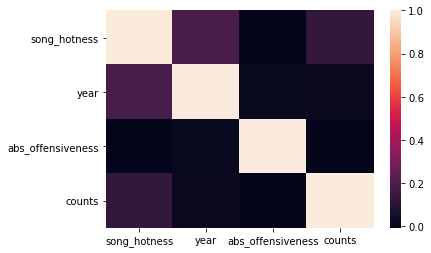
\includegraphics{plots/basic_correlations}
\caption{Basic correlations for all songs}
\label{basic_correlations}
\end{figure*}

We have investigated the effect of other scaling and filtering schemes, such as:

\begin{itemize}
\item we have tried using the logarithm of the play count instead of the original number of times the songs have been played. This was because the songs which were played often could have a huge value as compared to the ones which were played only 1, 2, 3, or a few times. We wanted to smooth those values so that the difference between popular and non popular songs can be better measured. Unfortunately this didn't give us better correlations than before. However we notice that the correlation between song hotness and play counts suddenly jumped from 0.13 to 0.51 so, at least, we got some insights about the way the song hotness was computed in the Million Songs dataset: they probably also used the logarithm of the play counts value as one of the measures of popularity.
\item We removed songs where the play count was very low hoping that the data was better for more popular songs. So we took only songs that were played at least 4 times. Unfortunately, we still didn't get any improvement out of this.
\item In the same spirit as the previous one we tried to keep only recent songs (we tried both with songs which were released after 1990 and those which were released after 2000). We hoped that the data was better for recent songs and that we could get some meaningful correlations with this strategy, but nothing: the correlations are still close to zero.
 \end{itemize}


\subsection{Correlations over time}
Since we didn't get meaningful correlations using all songs at once, it might be interesting to include the temporal dimension and try to figure out whether there are correlations for specific years. We show the results on figure \ref{correlation_time}.

\begin{figure*}
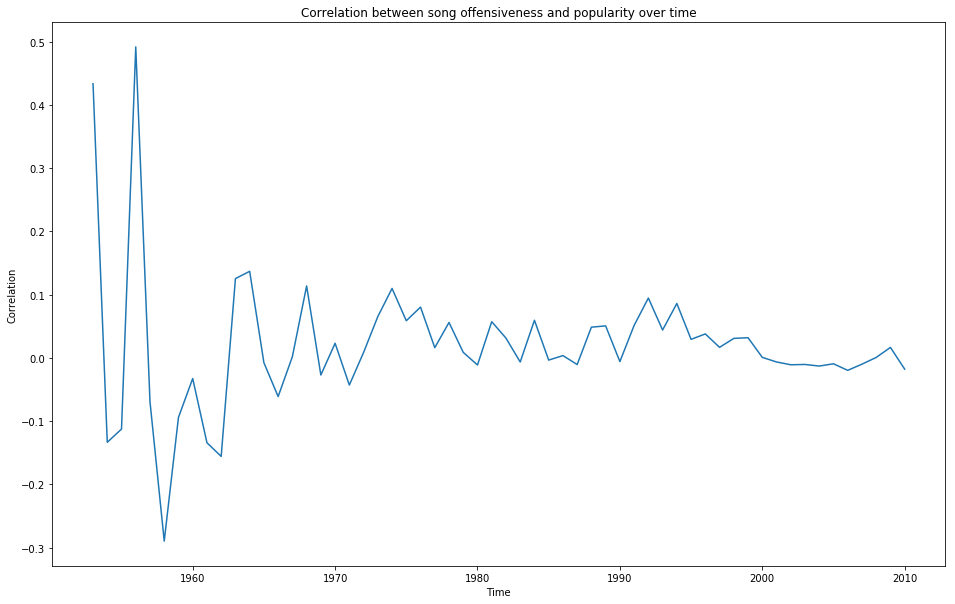
\includegraphics[width=\linewidth]{plots/correlation_time}
\caption{Correlation between song offensiveness and popularity over time}
\label{correlation_time}
\end{figure*}

As we see there are no correlations except in the beginning of the time period of the Million Song dataset. Unfortunately, we have very few songs for that time period and we tried to get more insights on them (see the chapter on the number of swear words approach). Before giving more details let us take a closer look at figure \ref{correlation_time_categories}. We have plotted the same correlations as before but this time we did this for some of the swear words categories.

\begin{figure*}
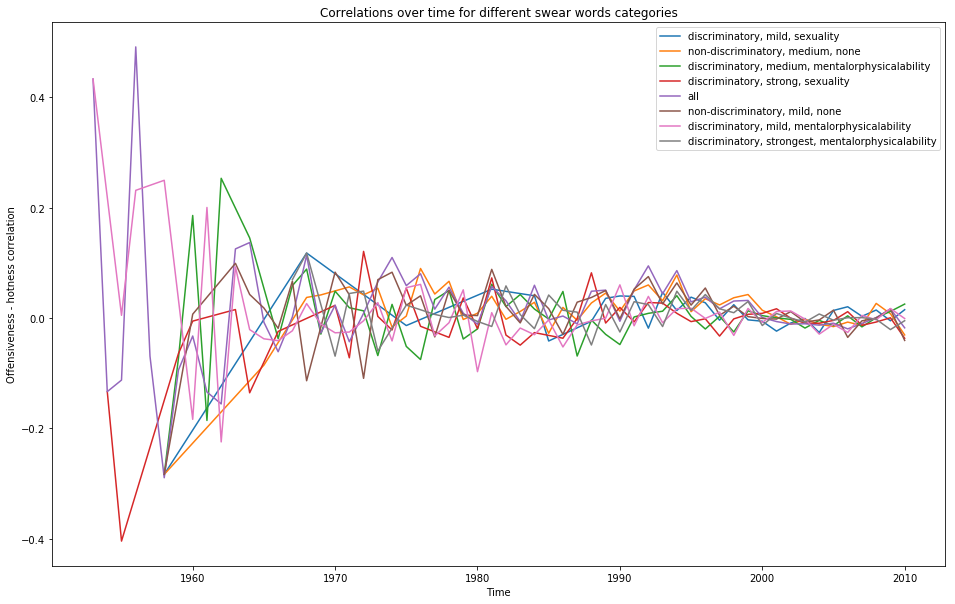
\includegraphics[width=\linewidth]{plots/correlation_time_categories}
\caption{Correlation between song offensiveness and popularity over time for different swear words categories}
\label{correlation_time_categories}
\end{figure*}

Again, we see the same trend as before. The plot has many colors but it is not so annoying since we clearly see that all curves (for all swear word categories) follow the same trends: they are very high in the first few years and then they tend to 0. We might be tempted to think that, for music in the mid-20th century, popularity is more correlated with offensiveness because of the Second World War but this is probably wrong. In the following we will see that we have very little data for those years; this leads to very strong correlations as soon as one song has one swear word. It is to be noted that our algorithms sometimes make mistakes because of the lyrics data we are provided with. We will see an example where the lyrics contain the words Whoo - hoo which doesn't mean anything but MusixMatch put the "hoo" as "ho", which is a swear word in our data.

\subsection{Data visualization}
Everything we did until now seems to show that there is no linear dependency for our data. 
But this does not mean there is no dependency at all. 
Another useful method to get better insights about data is to visualize it. 
We use a variety of scatter plots to search for structure in the data.
While this can help to show patterns, we would like to emphasize that the plots don't give any intuition for the actual density of the points.
The plots are on figure \ref{scatter_plots}.

\begin{figure*}
\begin{subfigure}[b]{0.45\textwidth}
\centering
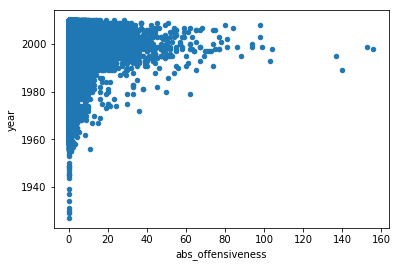
\includegraphics[width=\textwidth]{plots/scatter_off_time}
\caption{Offensiveness over time}
\label{scatter_off_time}
\end{subfigure}
\quad
\begin{subfigure}[b]{0.45\textwidth}
\centering
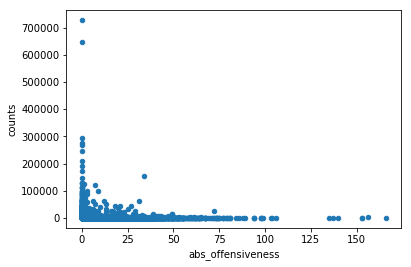
\includegraphics[width=\textwidth]{plots/scatter_off_counts}
\caption{Play counts vs offensiveness}
\label{scatter_off_counts}
\end{subfigure}

\centering
\begin{subfigure}[b]{0.45\textwidth}
\centering

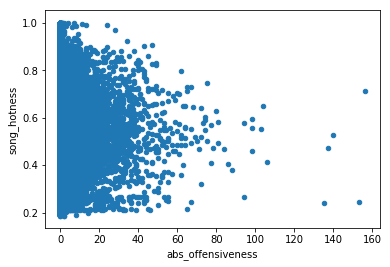
\includegraphics[width=\textwidth]{plots/scatter_off_hotness}
\caption{Popularity vs offensiveness}
\label{scatter_off_hotness}
\end{subfigure}
\caption{Scatter plots}
\label{scatter_plots}
\end{figure*}

We show the offensiveness compared to time (on figure \ref{scatter_off_time}), to play counts(on figure \ref{scatter_off_counts}) and to popularity/hotness (on figure \ref{scatter_off_hotness}). The median of absolute offensiveness is $2$ so we decided to also try to plot the same graphs for songs with 2 or more swear words on figure \ref{scatter_plots_2}. 

\begin{figure*}
\begin{subfigure}[b]{0.45\textwidth}
\centering
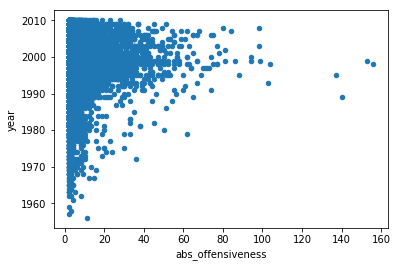
\includegraphics[width=\textwidth]{plots/scatter_off_time_2}
\caption{Offensiveness over time}
\label{scatter_off_time_2}
\end{subfigure}
\quad
\begin{subfigure}[b]{0.45\textwidth}
\centering
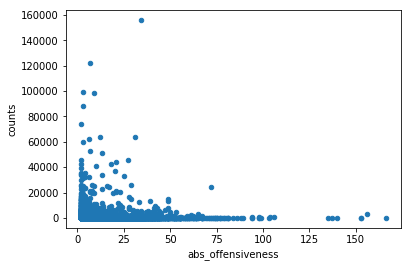
\includegraphics[width=\textwidth]{plots/scatter_off_counts_2}
\caption{Play counts vs offensiveness}
\label{scatter_off_counts_2}
\end{subfigure}

\centering
\begin{subfigure}[b]{0.45\textwidth}
\centering

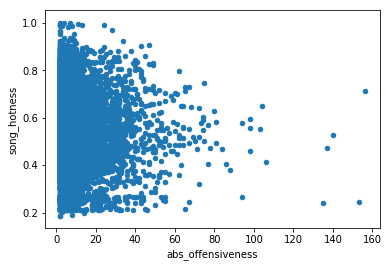
\includegraphics[width=\textwidth]{plots/scatter_off_hotness_2}
\caption{Popularity vs offensiveness}
\label{scatter_off_hotness_2}
\end{subfigure}
\caption{Scatter plots for songs with 2 or more offensive words}
\label{scatter_plots_2}
\end{figure*}

There is not much difference between the 2 scatter plots groups but we can see some structure in the data. First, we see that offensiveness increases over time. The most offensive period in music history is probably located in the last decade of the 20th century but it seems to decrease a little after that. As for the play counts, we can note that the songs which are the most listened to are in general not offensive and that play counts seem to decrease with offensiveness. But the most interesting plot is the hotness one on figures \ref{scatter_off_hotness} and \ref{scatter_off_hotness_2}. It shows that the average hotness songs tend to be more offensive than the others. We see this kind of vertical gaussian shape which seems to culminate somewhere around hotness $0.55$. The trends we observe are driven by a small subset of data points but the mass in center is useless. 


\subsection{Ratio approach}
In this section we introduce a new metric for analysing offensiveness over time: the ratio of offensive songs for a given year. We simply count all the offensive songs and divide it by the total number of song for that year. Our results are shown on figure \ref{ratio_time}. Of course we have to specify what it means for a song to be offensive. In our plots we simply put a threshold on the number of offensive words. On figure \ref{ratio_time} the threshold is $1$ so any song which contains at least one swear word will be considered as offensive. However, we try to vary that threshold and we show more general results on figure \ref{ratio_time_threshold}.

\begin{figure*}
\centering
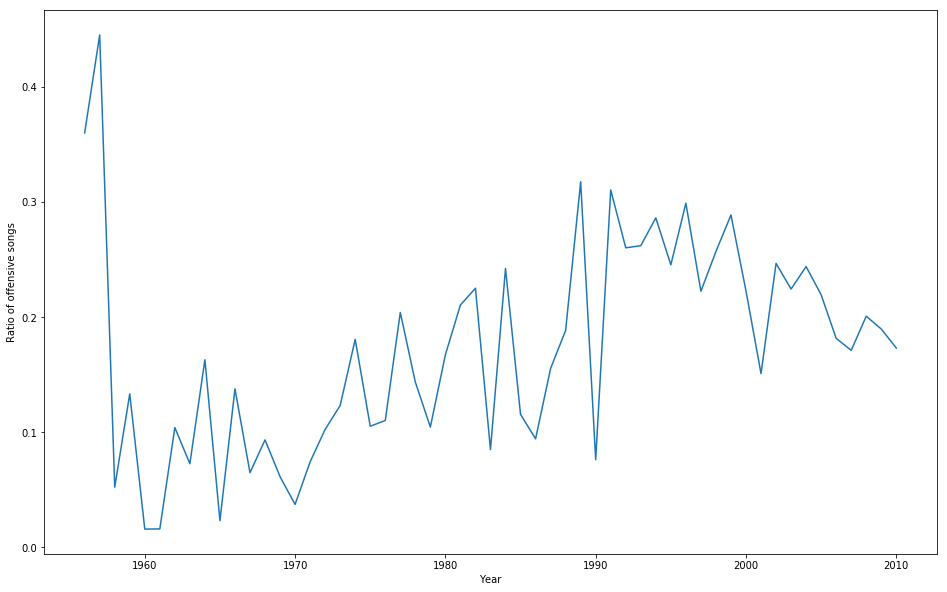
\includegraphics[width=\textwidth]{plots/ratio_time}
\caption{Ratio of offensive songs over time (threshold = 1)}
\label{ratio_time}
\end{figure*}

\begin{figure*}
\centering
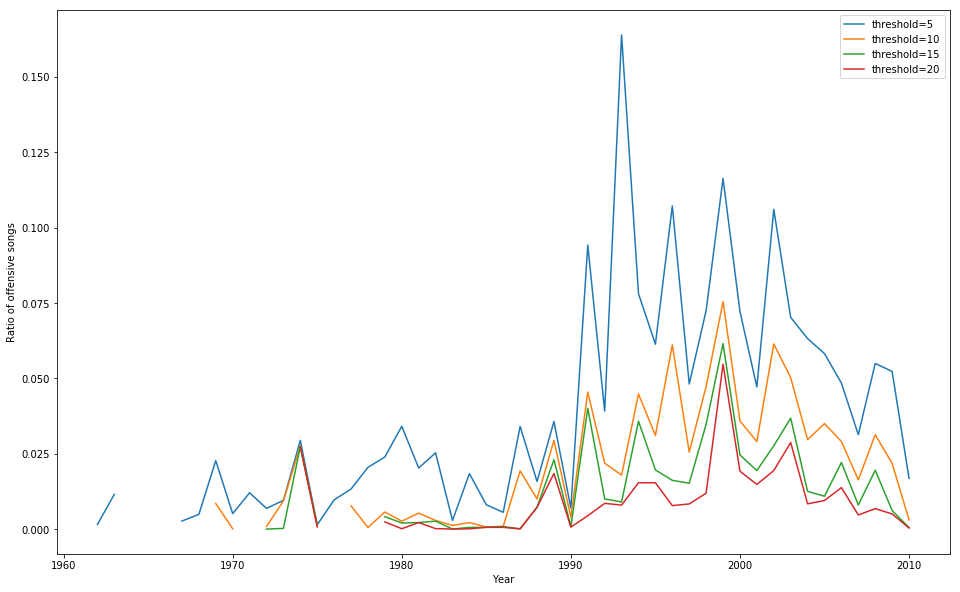
\includegraphics[width=\textwidth]{plots/ratio_time_threshold}
\caption{Ratio of offensive songs over time (higher thresholds)}
\label{ratio_time_threshold}
\end{figure*}

All the threshold seem to lead to a similar conclusion: the offensiveness trends start to spike in the 1990-2000 decade and then decrease when we enter the 21st century. They are nevertheless "kept alive" for a few more years after 2000 before starting to fade. This confirms our intuition from the scatter plots about offensiveness over time.

\subsection{Number of swear words approach}
Now what if we try to simply plot the number of offensive words without taking the songs themselves into account. We simply take all the lyrics for a given year, count the swear words and keep that result. You can observe what we obtain on figure \ref{nb_words}. Of course this is not the right measure since the number of total songs is varying over time so we show the average number of swear words per song on figure \ref{nb_words_avg}

\begin{figure*}
\centering
\begin{subfigure}[b]{0.45\textwidth}
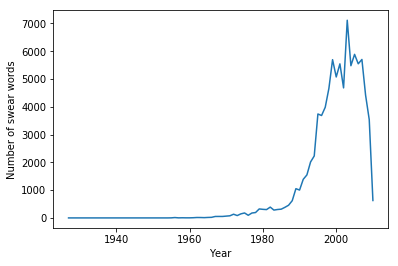
\includegraphics[width=\textwidth]{plots/nb_words}
\caption{Overall}
\label{nb_words}
\end{subfigure}
\quad
\begin{subfigure}[b]{0.45\textwidth}
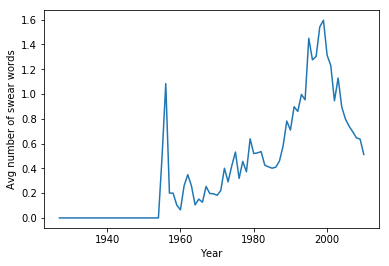
\includegraphics[width=\textwidth]{plots/nb_words_avg}
\caption{On average per song}
\label{nb_words_avg}
\end{subfigure}
\caption{Number of swear words}
\end{figure*}

Again, we are in the same situation as before: the offensiveness spikes in the last decade of the 20th century and then slowly starts to decrease after the year 2000. Do not be confused by the sudden spike in the year 1956. Actually it is due to a "bug" in the lyrics data. There are 12 songs for that year in our dataset and one of them, "Smokestack Lightning" by Howlin'Wolf, apparently contains 11 swear words. But if we look at the lyrics we see that there are absolutely no swear words in that song. The problem is that the chorus contains the onomatopeia "Whoo hooo" which doesn't mean anything by itself but was recorded by MusixMatch as the word "ho" which is a swear word !

In order to have better insights we show the most offensive songs in our dataset in table \ref{most_offensive_songs}. As we see we have some problems with the data since quite a small sample of these(half of them) has valid year and hotness attributes, which may be a reason why we did not obtain more interesting correlations. Anyway, it is interesting to note that our intuitions from before are confirmed even more now: the 1990-2000 decade is the most offensive period in terms of music. Even the ones for which we do not have the year seem to belong to that decade. If we look up on the Internet, we see that the most offensive one "Don't Gimme No H.A.N./?" was released in 1997. As for the popularity, our intuition is confirmed: there seems to be no correlation between popularity and offensiveness. In this sample we mostly have songs of average hotness, with a few exceptions above above the average ("Gangster Tripping" and "Acid 8000") and below ("Down For My N's" and "Booty Man (Remix)").

\begin{figure*}
\centering
\begin{tabular}{lrrrr}
\toprule
                     title &  year &  abs\_offensiveness &  song\_hotness &  counts \\
\midrule
   Don't Gimme No H.A.N./? &     0 &              166.0 &           NaN &      38 \\
         Gangster Tripping &  1998 &              156.0 &      0.711211 &    3326 \\
           Down For My N's &     0 &              153.0 &      0.246865 &      65 \\
              Bitch Niggas &  1999 &              153.0 &           NaN &      58 \\
                 Roll Call &  1989 &              140.0 &      0.528782 &     138 \\
        Can't Tell Me Shit &  1995 &              137.0 &      0.471971 &      26 \\
         Booty Man (Remix) &     0 &              135.0 &      0.239629 &     135 \\
        Stop Fuckin Wit Me &     0 &              106.0 &      0.415050 &     443 \\
                 Acid 8000 &  1998 &              104.0 &      0.648113 &     424 \\
    Lose A Hoe\_ Gain A Hoe &  1993 &              103.0 &      0.552007 &       1 \\
 Playa Ass Shit (Explicit) &  1999 &               99.0 &           NaN &       6 \\
            Fuck That Shit &  2003 &               98.0 &      0.554983 &     509 \\
\bottomrule
\end{tabular}

\caption{Most offensive songs}
\label{most_offensive_songs}
\end{figure*}

\subsection{Machine learning approach}

Since there seems to be no linear correlation in our data we wanted to try a multilayer perceptron which could potentially have more power and discover structure and non-linear correlations. We used the python keras library and constructed a simple neural network with 4 layers: one input activation and three dense layers. The loss function is the classical mean squared error function and we used the adam optimizer. For more details please have a look at our notebook. We used the year and the play counts as features and the offensiveness as labels. We smoothed the offensiveness using a logarithm so that we can make an easier distinction between high and low values. We also smoothed the play counts and mapped them to a range between $0$ and $1$ using min-max scaling. We also used min-max scaling for the year, where the min corresponds to $1927$ and the max to $2010$. We show the results on figure \ref{ml_off_time_pop}.

\begin{figure*}
\centering
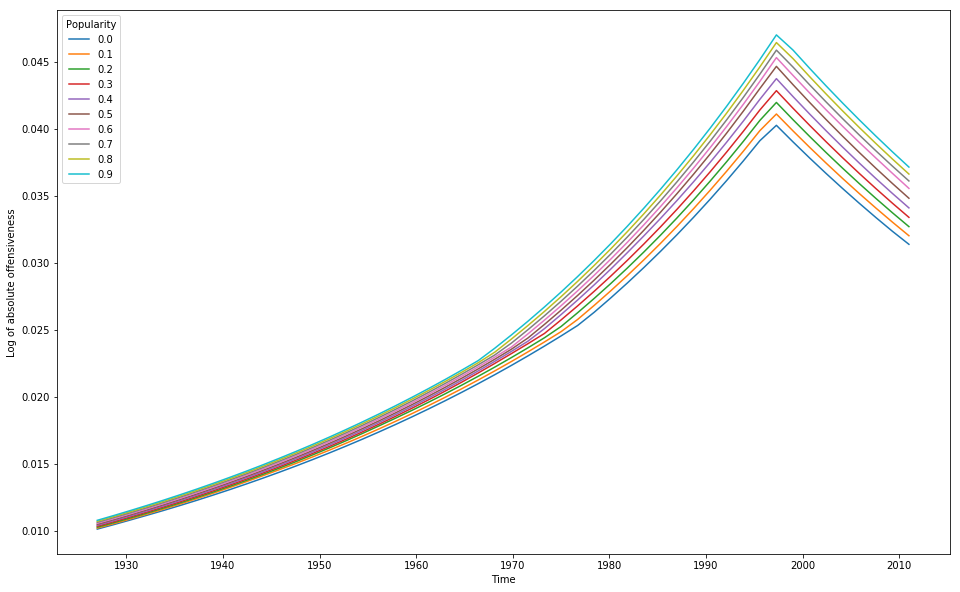
\includegraphics[width=\textwidth]{plots/ml_off_time_pop}
\caption{Offensiveness with popularity and time: machine learning approach}
\label{ml_off_time_pop}
\end{figure*}

As we can see, this approach also confirms the idea that songs were the most offensive in the 1990-2000 decade and that they became less vulgar after that. There still seems to be no or little dependency between popularity and offensiveness.

\section{Taking a step back: Criticism of the Datasets}
Our previous analysis has shown that there exists some trend over time concerning the offensiveness of songs. However, we have been surprised to discover that there seems to be no correlation between popularity and offensiveness. It is to be noted that no result might also be a result; it is possible that our research simply affirms that offensiveness doesn't influence the popularity of the songs. Nevertheless our exploration of the datasets lead us to believe that they are unreliable.
As an example, let's have a look again at the 10 most offensive songs in figure \ref{most_offensive_songs}.
From these 10 songs:
\begin{itemize}
  \item 2 have a hotness of NaN
  \item 4 have 0 as year of release
  \item the playcounts are highly questionable
  \item the hotness values are not coherent with the playcounts
\end{itemize}
Together the first two points remove 5 of the 10 songs. We have no workaround for the year of release, but the hotness can be replaced by the playcounts.\\
We take a closer look at the two songs "Bitch Niggas" and "Gangster Tripping". According to tasteprofile "Gangster Tripping", released by "Fat Boy Slim", has been played a total of 3326 times while "Bitch Niggas" has only a playcount of 58. This is hghly surprising since "Bitch Niggas" is the result of a collaboration between "Dr. Dre", "Snoop Dog" and "Mel Man", at least two of them being very popular.
We have searched for the two songs on Youtube and their view counts are very similar ("Bitch Niggas" is actually a little more popular).
On the other side, the playcounts indicate a much higher popularity for "Gangster Tripping".\\
In addition to the fact that the playcounts don't seem to be representative of the true relative popularity of the songs, the hotness values can be quite surprising. If we take a look at the song "Lose A Hoe Gain A Hoe", we see that it has a hotness of about $0.5$ and a playcount of $1$. On the other side, the song "Stop Fucking Wit Me", which has a playcount of $443$, has a lower hotness (about $0.4$)! These surprising results could simply be a consequence of the last evoked point: the playcounts are highly unreliable.\\ 
We are aware that such a cursory analysis is maybe not representative of the entire dataset.
However we do think that this warrants a new strategy and the search for alternative approaches.

\section{Results}
The correlation between offensiveness and popularity does not seem to exist. There is some structure for some of the songs but, in general, offensiveness seems to have little impact on popularity. There are as many very popular and offensive songs as there are offensive and unpopular ones. The correlation also seems to not exist over time or for the different swear words categories.\\
However, we still get a significant result: the offensiveness was on its peak in the last decade of the 20th century. This result is consistent throughout our different analysis methods. It is unsurprising knowing that this period was well known for the violence in the US "ghettos", where shootings and violence were very common. Rap music was an expression of this reality and it often expressed it using quite many offensive words. Despite everything, we are confident that we would have got better and more interesting insights if the datasets had been better.

\section{Outview}
In this outview we present alternative data sources that could be used to continue our research on the topic of music offensiveness and popularity.

\subsection{Youtube view count as popularity measure}
On first sight Youtube could be an excellent resource zo gain insights about the popularity of the different songs, using the view counts of the platform. Google even provides an official API to lookup such data.\\
The main problem is that Youtube was founded in 2005 so we would have no data for music before that
year. This would leave us with a lot of songs we can’t even talk about. And, since one of the core ideas of
our project is to do our analysis based on time (compute the correlations between offensiveness and
popularity over time), this would have left us with only a few years between 2005 and 2010 (the data
stops at 2011), which is probably not enough to do get interesting data.\\
Another issue tightly related to this one is that the popularity of the platform itself is variable. For example « Despacito » is the most viewed video on Youtube today with over 4.5 billion views but. Seven years ago, it was Justin Bieber’s « Baby » with only 1.7 billion views. Could we assess that « Despacito » is 2.6 times more popular than « Baby »? We would rather say that Youtube is much more used today. Fewer people had a (reliable) connection to the Internet. Simply said, there is a variable we might call « Youtube usage » (or poularity
or access) which varies over time and we would have to scale the number of views according to this variable.


Another problem we would encounter would be the matching of the songs between our dataset and Youtube. Our best option would simply be to try to match the names of our songs with the name on Youtube since the track id used in the Million Songs dataset simply does not exist on Youtube. However, we know there can be many videos
for one single song. We often have the official video and additional videos with lyrics posted by fans (and there
can be many of them). So the total number of views is spread across many videos and we have no guarantee that what we are querying is enough. We might only take official videos but even that is not a good idea because we would probably lose a lot of information and even if we didn't, how would we know what the official video is (looking for "official" in the title seems like an unreliable algorithm)?\\
Finally, it should be noted that the view count is not a good measure because a video can be removed and reuploaded (because of copyrights infractions for example).

\subsection{Spotify}
One other idea we had in mind was to use the Spotify API. Spotify is one of the most
popular apps today for listening to music so it can probably be used to gather interesting information. The
Spotify API is very complete since it provides us with all the values we would need in our analysis,
especially with the track information such as play counts for users or popularity. However, this popularity
attribute seems to vary over time because the documentation specifies that a song which has more play
counts now will have a better popularity than a song which has the same number of play counts in the
past. We might still use the play count in our analysis and it would probably give some
interesting results. However, the effort to put in this is too high because the process of registering an app to use the API seems to be quite long.

\subsection{Internet for the release year}
One of the main problems of our dataset is also that the year of realease is missing for a lot of songs. We believe this had a significant impact on our results. However, we can easily find the release year by searching the songs on Google. As such, one possibility might be to build a scraping system which would find the missing years. For example, it could do the search on Google, visit the sites and do natural language processing in order to find it. However, it is obvious that this strategy would be very difficult and time-consuming to set up. There would probably be a lot of exceptions where it would not work. The amount of effort and time put into this type of approach would probably not be worth the results. 

\begin{thebibliography}{}

  
\bibitem[\protect\citename{MSD}]{MSD}
\newblock {\em Million Song Dataset}
\newblock MSD
\newblock https://labrosa.ee.columbia.edu/millionsong/

\bibitem[\protect\citename{MusixMatch}]{MusixMatch}
MusixMatch Dataset, https://labrosa.ee.columbia.edu/millionsong/musixmatch

\bibitem[\protect\citename{Aho and Ullman}1972]{Aho:72}
Alfred~V. Aho and Jeffrey~D. Ullman.
\newblock 1972.
\newblock {\em The Theory of Parsing, Translation and Compiling}, volume~1.
\newblock Prentice-{Hall}, Englewood Cliffs, NJ.

\bibitem[\protect\citename{{American Psychological Association}}1983]{APA:83}
{American Psychological Association}.
\newblock 1983.
\newblock {\em Publications Manual}.
\newblock American Psychological Association, Washington, DC.

\bibitem[\protect\citename{{Association for Computing Machinery}}1983]{ACM:83}
{Association for Computing Machinery}.
\newblock 1983.
\newblock {\em Computing Reviews}, 24(11):503--512.

\bibitem[\protect\citename{Chandra \bgroup et al.\egroup }1981]{Chandra:81}
Ashok~K. Chandra, Dexter~C. Kozen, and Larry~J. Stockmeyer.
\newblock 1981.
\newblock Alternation.
\newblock {\em Journal of the Association for Computing Machinery},
  28(1):114--133.

\bibitem[\protect\citename{Gusfield}1997]{Gusfield:97}
Dan Gusfield.
\newblock 1997.
\newblock {\em Algorithms on Strings, Trees and Sequences}.
\newblock Cambridge University Press, Cambridge, UK.

\end{thebibliography}

\end{document}
